%!TEX program = xelatex
% Encoding: UTF8
% SEIKA 2018
% Author weizhou

\documentclass[a4paper,11pt,oneside]{ctexbook}

\usepackage{makeidx}
\makeindex

\usepackage{geometry}
\geometry{left=3.5cm, right=3cm, top=3cm, bottom=3cm}
%控制页眉页脚页码
\pagestyle{plain}
%罗马字符页码
%\pagenumbering{roman}

% 支持西文字体
\usepackage{fourier}
\usepackage{courier}
% \usepackage{fontspec}

\newfontfamily\CodeFont{Consolas}

\usepackage{graphicx}

\usepackage{booktabs}

\usepackage{amssymb}
\usepackage{amsfonts}

% 支持代码框插入
\usepackage{xcolor}
\definecolor{mygreen}{rgb}{0,0.6,0}
\definecolor{mygray}{rgb}{0.5,0.5,0.5}
\definecolor{mymauve}{rgb}{0.58,0,0.82}
\definecolor{codeback}{rgb}{1, 0.99, 0.87}
\definecolor{etc}{rgb}{0.24,0.07,0.18}
\definecolor{etc}{rgb}{0.54,0.37,0.48}
\definecolor{language-c-keyword-color}{rgb}{0.0,0.0,1.0}
\definecolor{language-c-struct-color}{rgb}{0.0,0.5,0.0}
\definecolor{oam-pkt-flag}{rgb}{0.5, 0.8, 0.0}
\definecolor{oam-pkt-opcade}{rgb}{0.0, 0.0, 0.9}
\definecolor{oam-pkt-oui}{rgb}{0.9, 0.0, 0.0}
\definecolor{oam-pkt-branch1}{rgb}{0.8, 0.3, 0.0}
\definecolor{oam-pkt-branch2}{rgb}{0.8, 0.5, 0.0}
\definecolor{oam-pkt-branch3}{rgb}{0.8, 0.8, 0.0}

\def\degree{${}^{\circ}$}

\usepackage{amsmath}

\usepackage[misc]{ifsym}

% 支持超链接
\usepackage[colorlinks]{hyperref}

\usepackage{listings}
\lstset{ %
  backgroundcolor=\color{codeback},    % choose the background color; you must add \usepackage{color} or \usepackage{xcolor}
  basicstyle=\linespread{0.95}\footnotesize\CodeFont,   % the size of the fonts that are used for the code
  breakatwhitespace=false,           % sets if automatic breaks should only happen at whitespace
  breaklines=true,                   % sets automatic line breaking
  captionpos=bl,                     % sets the caption-position to bottom
  commentstyle=\color{mygreen},      % comment style
  deletekeywords={...},              % if you want to delete keywords from the given language
  escapeinside={\%*}{*)},            % if you want to add LaTeX within your code
  extendedchars=true,                % lets you use non-ASCII characters; for 8-bits encodings only, does not work with UTF-8
  frame=single,                      % adds a frame around the code
  frameround=tttt,
  keepspaces=true,                   % keeps spaces in text, useful for keeping indentation of code (possibly needs columns=flexible)
  keywordstyle=\color{blue},         % keyword style
  language=XML,                    % the language of the code
  morekeywords={*,...},              % if you want to add more keywords to the set
  numbers=left,                      % where to put the line-numbers; possible values are (none, left, right)
  numbersep=4pt,                     % how far the line-numbers are from the code
  numberstyle=\tiny\CodeFont\color{mygray},   % the style that is used for the line-numbers
  rulecolor=\color{mygray},          % if not set, the frame-color may be changed on line-breaks within not-black text (e.g. comments (green here))
  showspaces=false,                  % show spaces everywhere adding particular underscores; it overrides 'showstringspaces'
  showstringspaces=true,             % underline spaces within strings only
  showtabs=true,                     % show tabs within strings adding particular underscores
  stepnumber=1,                      % the step between two line-numbers. If it's 1, each line will be numbered
  stringstyle=\color{orange},        % string literal style
  tabsize=2,                         % sets default tabsize to 2 spaces
  %title=myPython.py                 % show the filename of files included with \lstinputlisting; also try caption instead of title
  xleftmargin = 1em,
  xrightmargin = 1em,
  aboveskip = 0.5 em
}

\lstdefinestyle{styleC}{
    language=C,
    keywordstyle=\color{language-c-keyword-color}\bfseries,
    commentstyle=\color{blue} \textit,
    showstringspaces=false,
    numbers=left,
    numberstyle=\tiny\CodeFont\color{mygray},
    morekeywords={try, except},
    emph={
      csComStackInit_t, csInitVehicleData_CycCalbk_t, csLog_pFun, MCP2515_CAN_FILTER_CTL
    },
    emphstyle=\color{language-c-struct-color},
}

\lstdefinestyle{stylePy}{
    language=Python,
    keywordstyle=\color{language-c-keyword-color}\bfseries,
    commentstyle=\color{blue} \textit,
    showstringspaces=false,
    numbers=left,
    numberstyle=\tiny\CodeFont\color{mygray},
    morekeywords={try, except},
}

%%%%%%%%%%%%
\title{message router design}
\author{weizhou\thanks{awokezhou@gmail.com}}
\date{\today}

\begin{document}

\maketitle
\tableofcontents

\chapter{引言}
在Linux应用层开发过程中,通常以进程的方式完成某项特定功能。系统中会同时运行多个进程,而根据业务的需要,进程间需要相互通信几乎是必须的。Linux为进程间通信提供了几种原始的方法:管道和命名管道、信号、信号量和unix socket。多进程间传递消息经常被使用的是unix socket,其他几种方式从设计理念和目的上不适合用来进行多进程间大量消息的传输。

要使用unix socket,每个进程必须创建一个socket绑定一个文件作为本地通信的地址,如图1.1所示。

\begin{figure}[ht]
    \centering
    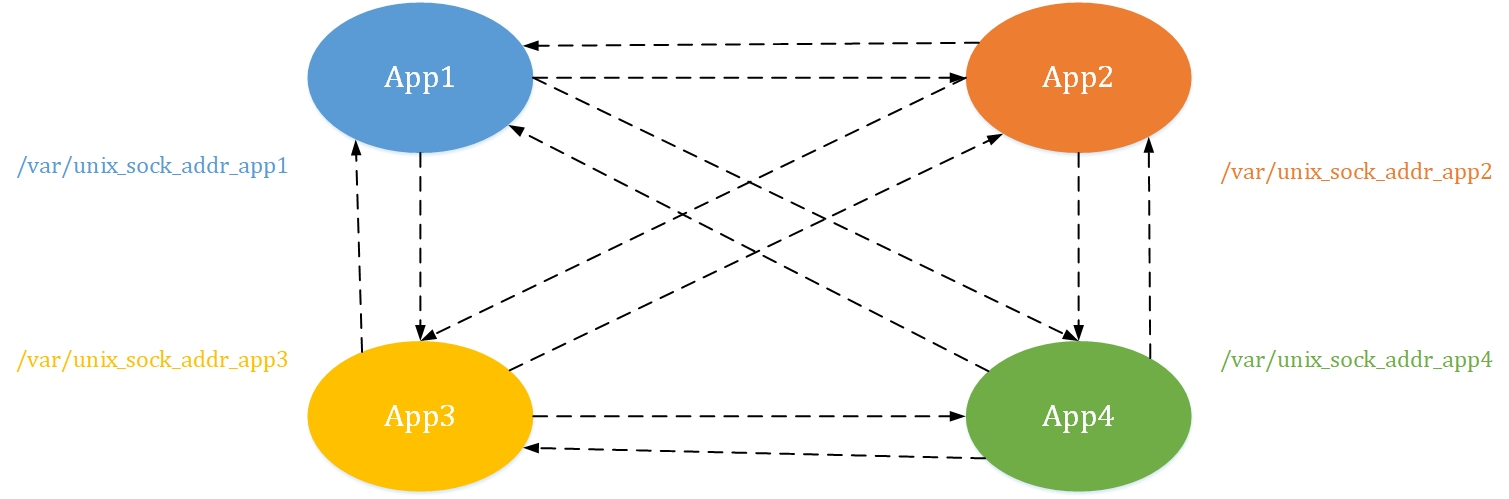
\includegraphics[width=1\textwidth]{image/message-router-01.jpg}
    \caption{多进程使用unix socket通信}
\end{figure}

如果多个应用要进行复杂的交互,那么需要为此创建多个地址文件,这虽然对于Linux系统来说不是什么难题,但是这样的通信模型对于应用软件的设计、开发和维护来说,都太过复杂和不必要。另外,如果某个应用想要想其他多个应用发送类似组播或者广播消息,这种通信结构就更加难以维护。

基于以上的问题和需求,提出消息路由(message route)的概念,即创建一个消息中转站,类似通信中的路由器,能够对消息做转发,所有进程间的消息通信,都统一发送到中转站,再由中转站根据消息的目的地址发往目的进程。如图1.2所示。

消息路由的设计仅限于本地通信的各个进程之间,并不包括远程服务和代理,其设计属于集中式结构,而不是分布式结构,需要一个专门用于提供中转服务的进程router来做消息转发,定义一个公共库librtmsg来规范各个进程的消息格式、发送和接收处理。而各个进程的消息通信ID必须预先在router中固定编写,不支持进程上线后临时上报,即未在router中记录的进程无法使用message route来转发消息。

\newpage
\begin{figure}[ht]
    \centering
    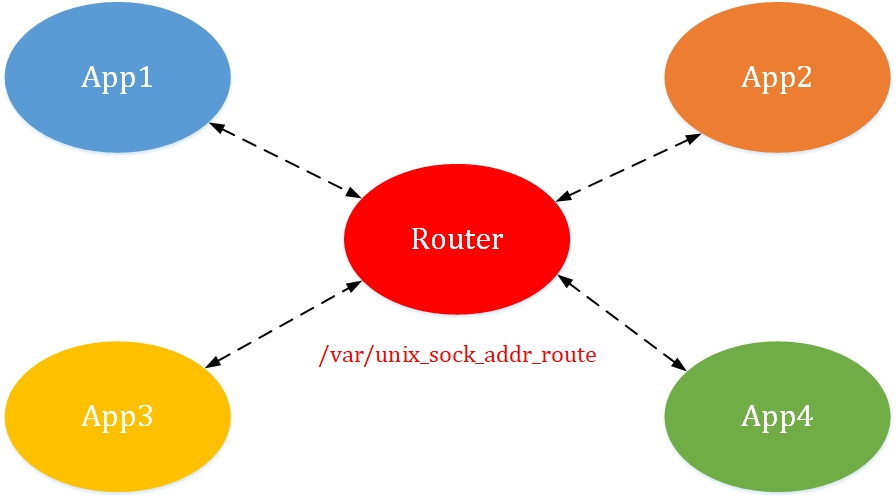
\includegraphics[width=0.7\textwidth]{image/message-router-02.jpg}
    \caption{message route}
\end{figure}

本文章节安排如下:

1. 第二章对整个message route的处理流程进行描述,包括router如何初始化、进程与router的交互、router的消息转发。

2. 第三章对librtmsg中的主要内容进行说明,包括App信息表、公共API。

2. 第四章对消息格式进行定义。

\chapter{message route消息处理流程}

\section{router init}
首先有一个非常关键的点,router的启动必须先于需要使用message route机制转发消息的其他进程,因为消息转发的核心在于unix socket的建立,如果unix socket还未建立之前其他进程就已经开始尝试转发消息,这是不好的设计,也是不安全的(导致进程阻塞)。当然你也可以将其他进程connection动作设置为非阻塞的,但是这样的设计从根本上是劣质的。创建unix socket的任务理所应当放在了router中完成。

要进行消息转发,需要在中转站上存放一个中转表,就像交换机上有MAC Table,路由器上有Route Table一样,router中也需要一个转发表(forward table, fdt)。想象一个最简单的模型,当一个进程App1要向进程App2发送消息时,App1的消息中必定包含了发往进程的目的标识dst id,此消息发送到router后,router将根据这个dst id在转发表fdt中查找,获取对应进程的消息句柄msg handle,以该句柄向App2发送消息。如图2.1所示。

\begin{figure}[ht]
    \centering
    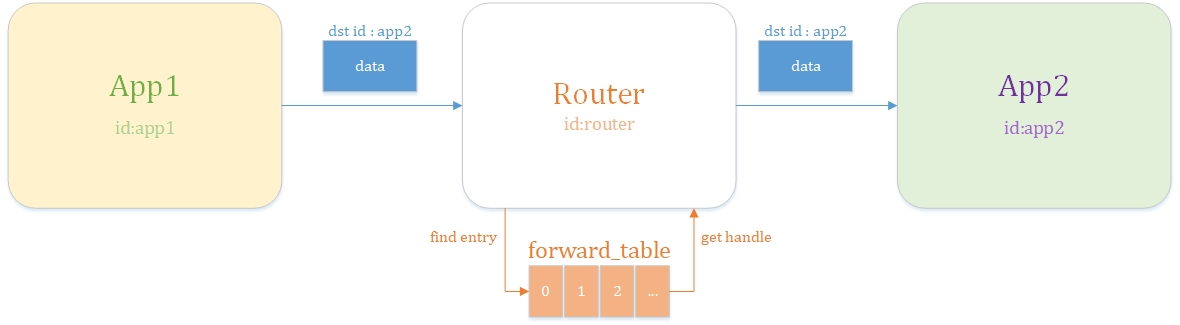
\includegraphics[width=1\textwidth]{image/message-router-03.jpg}
    \caption{两个进程消息通信}
\end{figure}

那么转发表如何生成呢?其中的每一个表项存放什么内容呢?目前转发表固定写死在librtmsg库中,以静态数组呈现,router初始化时将其中的每一个表项添加到自己的转发表中。以上文的分析,每个表项至少应该存放进程标识id,和消息句柄msg handle。

因此,router的初始化关键的两个步骤:

\begin{itemize}
  \item{创建unix socket}
  \item{初始化转发表}
\end{itemize}

\section{router running time}
当router以上述方式初始化完成后,则在unix socket上监听消息,但是此时如果直接进行消息转发,则存在以下两个问题:

\begin{itemize}
  \item{如果消息转发的目的App未启动,则会转发失败}
  \item{初始消息转发的目的App未和router建立连接,router没有获取到App的消息句柄,转发也会失败}
\end{itemize}

以上问题总结来说,就是只有消息通信App双方都已经启动,并且与router建立了连接,才可以进行消息转发,那么如何解决呢?router需要对进程的状态进行记录和管理,转发表的表项中需要对App的状态有所记录,当App与router建立连接后,转发表中对应此App的表项将App状态变为可转发的,然后将此App的消息句柄记录。当App的状态得到记录,并且消息句柄存在时,就可以进行正常的转发了。router根据消息结构中的目的标识将此消息转发给目的App。

router运行时处理流程如图2.2所示。

\begin{figure}[ht]
    \centering
    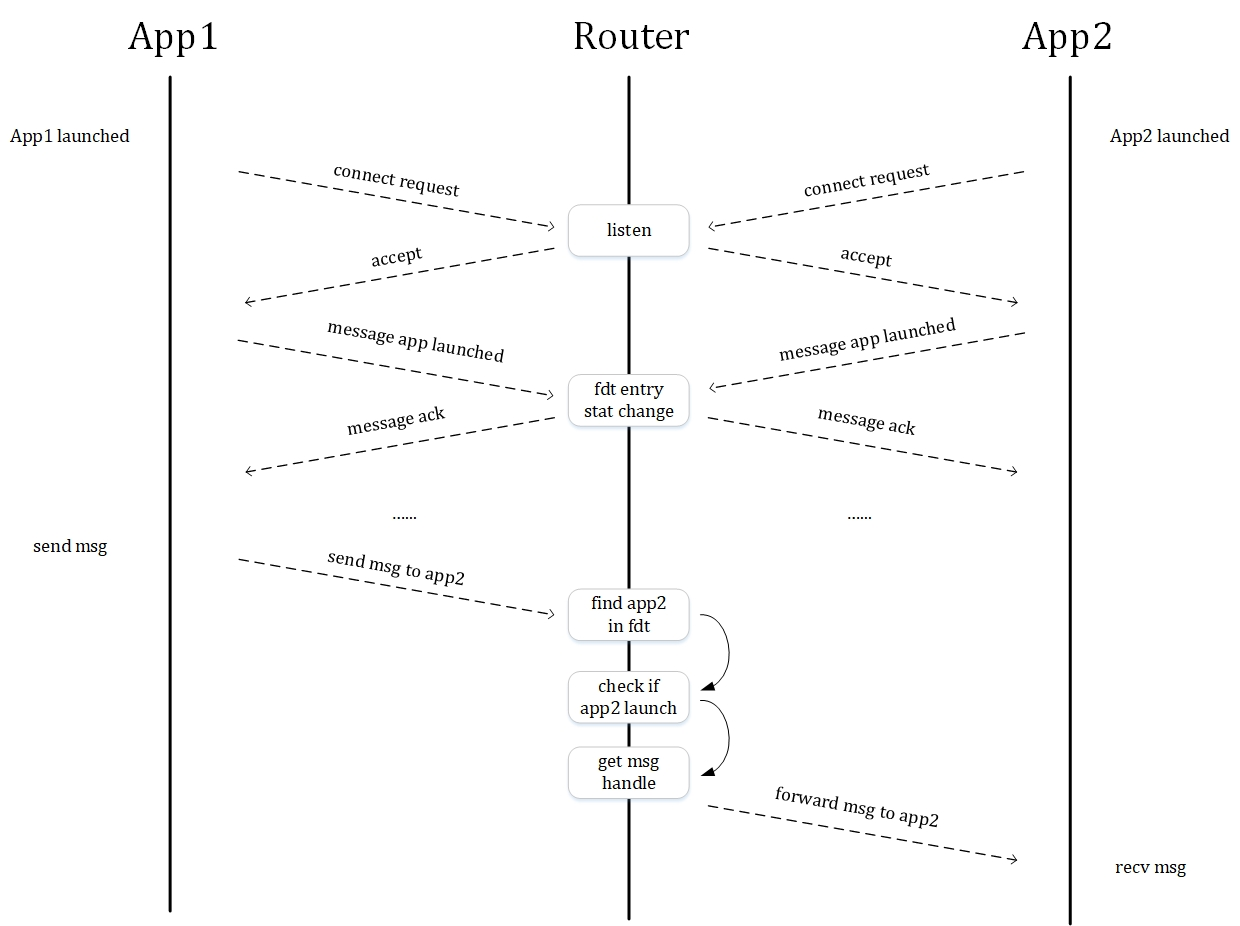
\includegraphics[width=1\textwidth]{image/message-router-04.jpg}
    \caption{router运行时逻辑}
\end{figure}

\chapter{librtmsg}
\section{进程ID和信息定义}
librtmsg库中以静态数组的方式定义一个进程信息表app\_info\_array,每个进程包括一个唯一标识app\_id,一个进程名称,一个进程标志(保留)。进程标识app\_id以整形数字的形式存在。

\end{document}
